\chapter{Laboratorio 4}
\section{Introduzione}
Durante questa attività di laboratorio si è dapprima terminata l'analisi per piccolo segnale del circuito common emitter amplifier e in seguito si è introdotto l'utilizzo del amplificatore operazionale \textmu A741 (datasheet:\url{https://www.ti.com/lit/ds/symlink/ua741.pdf}), utilizzato nella configurazione di amplificatore invertente e integratore reale.

\section{Common emitter amplifier: analisi capacità di disaccoppiamento in ingresso}
Si ricordi l'analisi di piccolo segnale del circuito common emitter amplifier con alimentazione singola già presentata (capitolo \ref{sec:33}), considerando però ora anche la capacità di disaccoppiamento C (\Fig\ref{fig:commonemitter_se_c_AC}).
\begin{figure}[h!]
	\centering
	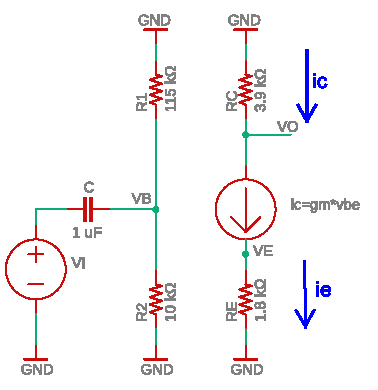
\includegraphics[width=0.4\linewidth]{./OtherFiles/Laboratorio 4/common emitter_se_c-piccolo segnale-printout}
	\caption{Analisi per piccolo segnale del circuito common emitter amplifier con alimentazione singola.}
	\label{fig:commonemitter_se_c_AC}
\end{figure}

\noindent
Le resistenze R\sub{1} e R\sub{2} sono in parallelo, poiché connesse tra il nodo v\sub{b} e massa. Esse possono quindi essere sostituite con una resistenza equivalente di valore $R_{12}=R_1 // R_2=\frac{R_1 R_2}{R_1+R_2}$. Svolgendo un bilancio di correnti al nodo v\sub{b}, siamo in grado di definire l'andamento della tensione nel nodo v\sub{b} nel dominio delle trasformate di Laplace:
\begin{equation}
	\begin{split}
		i_C(s)&=i_R(s) \\
		\frac{v_i(s)-v_b(s)}{Z_C(s)}&=\frac{v_b(s)-\SI{0}{\volt}}{R_{12}} \\
		\frac{v_i(s)-v_b(s)}{\frac{1}{sC}}&=\frac{v_b}{R_{12}} \\
		(v_i(s)-v_b(s))sC&=\frac{v_b(s)}{R_{12}} \\
		\text{da cui} & \text{ si ricava per s=jw} \\
		v_b(jw)&=\frac{jwR_{12}C}{1+jwR_{12}C}v_i(jw).
	\end{split}
\end{equation}
L'equazione ricavata corrisponde all'equazione di un filtro passa-alto. Per cui, se $w>>w_C=\frac{1}{R_{12}C}$ allora v\sub{b}=v\sub{i}, ossia il condensatore può essere considerato un corto. Calcolando la pulsazione critica w\sub{C} con i valori delle resistenze del nostro circuito otteniamo $w_C\simeq \SI{107.5}{\radian/\second}$ che equivale a una frequenza di $f_C\simeq\SI{17.1}{\hertz}$.

Di seguito è riportato il diagramma di Bode reale del modulo della funzione di trasferimento che lega v\sub{i} e v\sub{b} (\Fig\ref{fig:hpf}). Dal grafico si può ricavare che la w\sub{C} è di \SI{109}{\radian/\second}, simile a quella calcolata in modo approssimativo. 
\begin{figure}[h!]
	\centering
	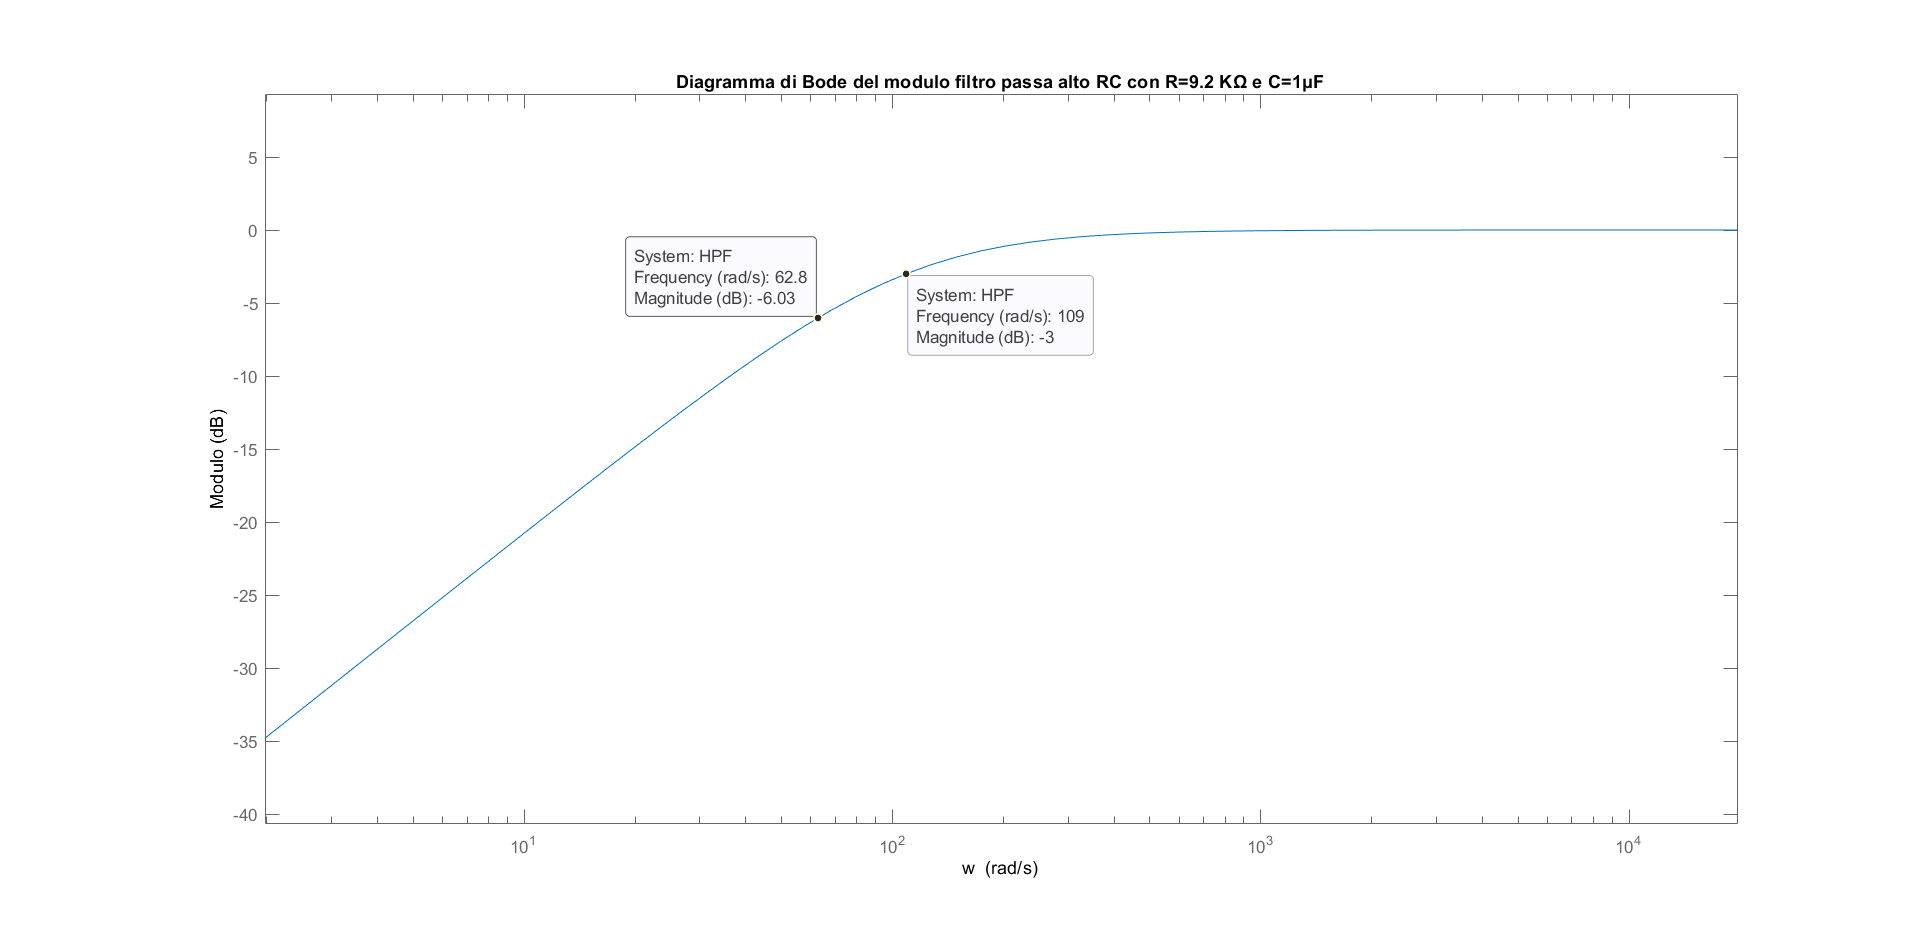
\includegraphics[width=1\linewidth]{./OtherFiles/Laboratorio 4/boderc.png}
	\caption{Diagramma di Bode del modulo del filtro RC passa-alto, con R=\SI{9.2}{\kilo\ohm} e C=\SI{1}{\micro\farad}.}
	\label{fig:hpf}
\end{figure}

\noindent
In laboratorio è stato possibile misurare la tensione al nodo v\sub{i} in ingresso e la tensione sul nodo v\sub{b}, con un segnale sinusoidale di frequenza \SI{10}{\hertz} e ampiezza picco-picco di \SI{100}{\milli\volt}. Nella figura \ref{fig:hpf_10hz} sono riportati i risultati. Lavorando ad una frequenza (che equivale a una pulsazione $w\simeq\SI{62.8}{\radian/\second}$) inferiore alla frequenza critica del filtro, il segnale è attenuato di circa \SI{4.2}{\decibel}. Inoltre, l'acquisizione risulta essere molto rumorosa, in quanto l'oscilloscopio presenta difficoltà nel misurare segnali con frequenza così bassa. Tuttavia, questo risultato è compatibile con il digramma di Bode del modulo sopra mostrato, il quale indica un valore di attenuazione pari a \SI{-6}{\decibel}. Inoltre, si può notare anche uno sfasamento tra i segnali in ingresso e in uscita introdotto dal filtro passa alto.
\begin{figure}[h!]
	\centering
	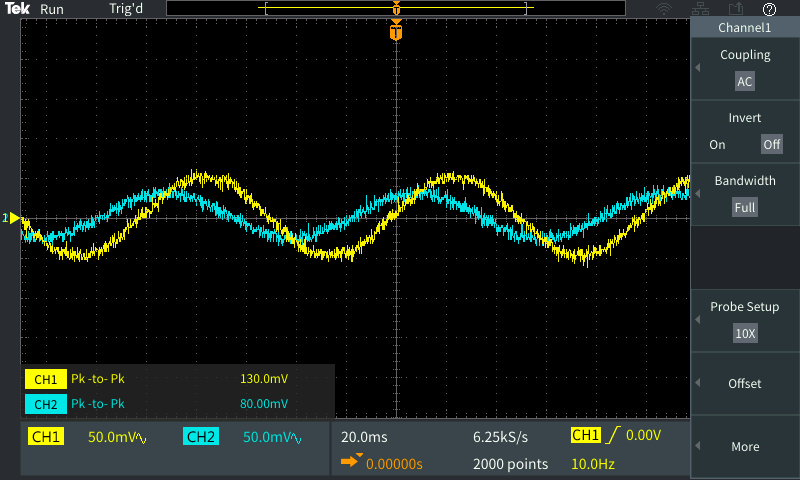
\includegraphics[width=0.7\linewidth]{./ImageFiles/Laboratorio 4/TEK00003}
	\caption{Confronto tra il segnale in ingresso (CH1) al condensatore e in uscita (CH2) sul nodo v\sub{i} con segnale sinusoidale di ampiezza picco-picco \SI{100}{\milli\volt} e frequenza \SI{10}{\hertz}.}
	\label{fig:hpf_10hz}
\end{figure}

\section{Amplificatore operazionale \textmu A741: amplificatore invertente}
Nella successiva esperienza di laboratorio, si è realizzato un amplificatore invertente utilizzando l'amplificatore operazionale \textmu A741, realizzando il seguente circuito:
\begin{figure}[h!]
	\centering
	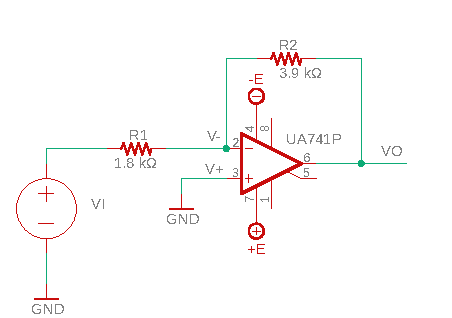
\includegraphics[width=0.6\linewidth]{./OtherFiles/Laboratorio 4/opam_inv}
	\caption{Amplificatore operazionale\textmu A741 in configurazione invertente.}
	\label{fig:opamp_inv}
\end{figure}

\begin{figure}[h!]
	\centering
	\includegraphics[width=0.6\linewidth]{./ImageFiles/Laboratorio 4/IMG\_20220531\_113527\_2}
	\caption{Circuito realizzato in laboratorio con l'amplificatore operazionale \textmu A741 in configurazione invertente.}
	\label{fig:opamp_inv_circuito}
\end{figure}

\noindent
In particolare, per le resistenze R\sub{1} e R\sub{2} sono state utilizzate le resistenze R\sub{C} e R\sub{E} utilizzate nel circuito precedente. Le tensioni di alimentazione +E e -E sono state inizialmente impostate a \SI{+10}{\volt} e \SI{-10}{\volt}.

\noindent
Analizzando il circuito, è facilmente ricavabile che 
\begin{equation}
	V_o=-\frac{R_2}{R_1}V_i,
\end{equation}
tramite un bilancio di corrente nel nodo V\textsuperscript{+} e ricordando che, in presenza di una reazione negativa, V\textsuperscript{+}=V\textsuperscript{-}. Con i valori di resistenze utilizzate, ci aspettiamo un guadagno di circa 2.17. Infatti, le misure effettuate tramite l'oscilloscopio rilevano un guadagno pari a circa 2.12 (\Fig\ref{fig:opamp_inv_amp}). Inoltre, il segno meno nella funzione di trasferimento ci indica che i segnali di ingresso e uscita devono risultare sfasati di \SI{180}{\degree}.
\begin{figure}[h!]
	\centering
	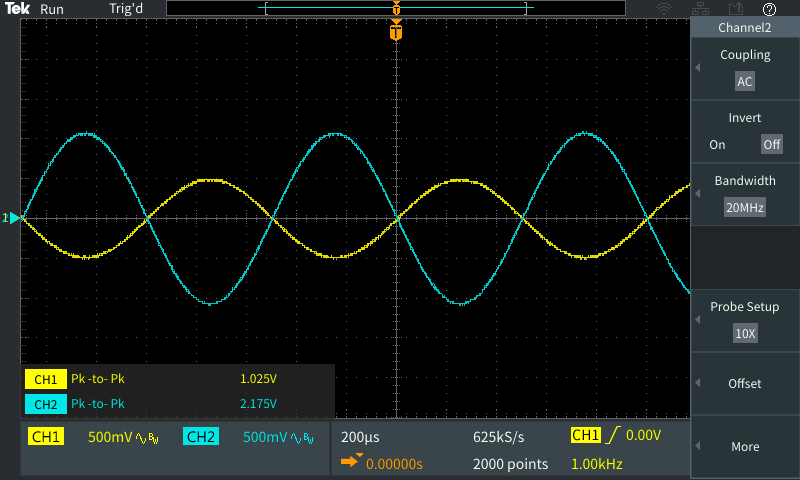
\includegraphics[width=0.7\linewidth]{./ImageFiles/Laboratorio 4/TEK00005}
	\caption{Confronto tra il segnale in ingresso v\sub{i} (CH1)  e in uscita v\sub{o} (CH2) con segnale sinusoidale di ampiezza picco-picco \SI{2}{\volt} e frequenza \SI{1}{\kilo\hertz}.}
	\label{fig:opamp_inv_amp}
\end{figure}

\noindent
Sostituendo le tensioni di alimentazione con +E=\SI{+5}{\volt} e -E=\SI{-5}{\volt}, si è provato a misurare la risposta del circuito a segnali in ingresso con ampiezza via via crescente da \SI{3}{\volt} fino a \SI{6}{\volt}. I risultati sono mostrati in figura \ref{fig:opamp_inv_sat}.
\begin{figure}[h!]
	\centering
	A
	\vspace{0.5cm}
	
	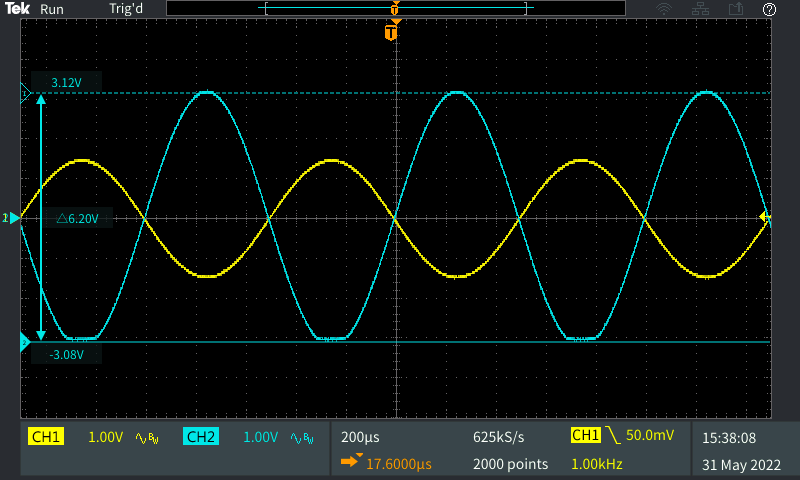
\includegraphics[width=0.7\linewidth]{./ImageFiles/Laboratorio 4/TEK00008}
	
	B
	\vspace{0.5cm}
	
	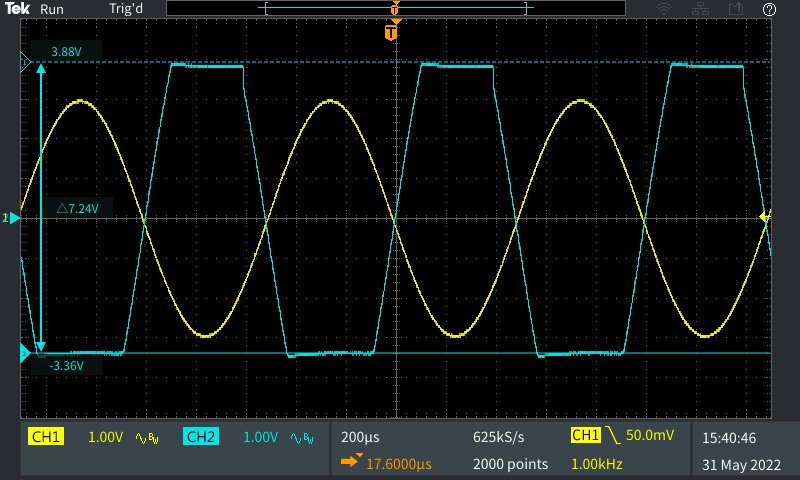
\includegraphics[width=0.7\linewidth]{./ImageFiles/Laboratorio 4/TEK00012}
	\caption{Confronto tra il segnale in ingresso v\sub{i} (CH1)  e in uscita v\sub{o} (CH2) con segnale sinusoidale di ampiezza picco-picco \SI{3}{\volt} (A) e \SI{6}{\volt} (B) e frequenza \SI{1}{\kilo\hertz}.}
	\label{fig:opamp_inv_sat}
\end{figure}
\`E possibile notare il fenomeno della saturazione. Infatti, la tensione in uscita da un amplificatore operazione non può mai superare le tensioni di alimentazione positiva e negativa (qui fissate a \SI{+-5}{\volt}). In realtà, si nota come la tensione di saturazione positiva e negativa in un operazionale reale sono addirittura inferiori alle tensioni di alimentazione (nel nostro caso circa \SI{4}{\volt} e \SI{-3.3}{\volt}). Un altro modo per visualizzare le tensioni limite di saturazione è quello di utilizzare in ingresso un onda triangolare e visualizzare l'andamento della tensione in uscita (\Fig\ref{fig:opamp_inv_sat_tri}).
\begin{figure}[h!]
	\centering
	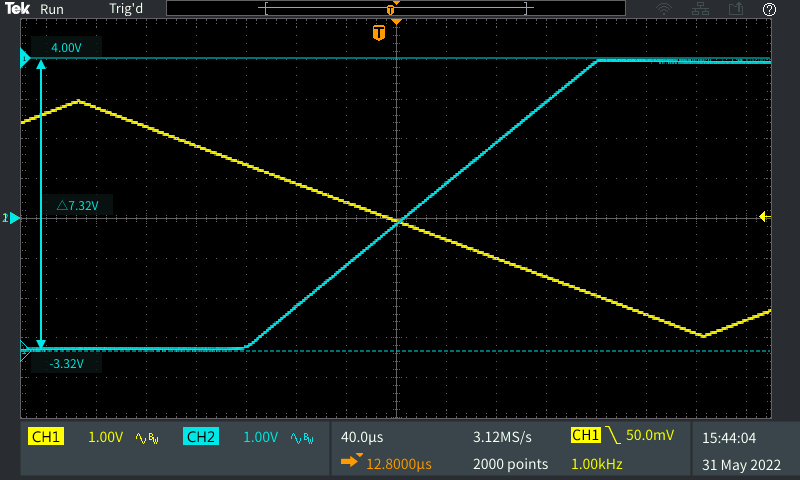
\includegraphics[width=0.7\linewidth]{./ImageFiles/Laboratorio 4/TEK00015}
	\caption{Confronto tra il segnale in ingresso v\sub{i} (CH1)  e in uscita v\sub{o} (CH2) con segnale triangolare di ampiezza picco-picco \SI{6}{\volt} e frequenza \SI{1}{\kilo\hertz}.}
	\label{fig:opamp_inv_sat_tri}
\end{figure}

\noindent
Si osservi come le tensioni di saturazioni non sono simmetriche, come spesso accade in amplificatori operazionali reali.

\clearpage
\section{Amplificatore operazionale \textmu A741: integratore}

L'ultimo circuito analizzato in laboratorio permette di realizzare un integratore reale:
\begin{figure}[h!]
	\centering
	\includegraphics[width=0.7\linewidth]{./OtherFiles/Laboratorio 4/opam\_int}
	\caption{Circuito con l'amplificatore operazionale \textmu A741 in configurazione di integratore.}
	\label{fig:opamp_int}
\end{figure}

\noindent
\`E possibile ricavare la funzione di trasferimento del circuito tramite un bilancio di correnti nel nodo V\super{-}, ricordando che essendo l'amplificatore in retroazione negativa, vale che V\super{+}=V\super{-}=\SI{0}{\volt}:
\begin{equation}
	\begin{split}
		I_{R_1}&=I_{C}+I_{R_2} \\
		\frac{V_i(s)-V^-(s)}{R_1}&=(V^-(s)-V_o(s))sC+\frac{V^-(s)-V_o(s)}{R_2} \\
		\frac{V_i(s)-\SI{0}{\volt}}{R_1}&=(\SI{0}{\volt}-V_o(s))sC+\frac{\SI{0}{\volt}-V_o(s)}{R_2} \\
		&\text{da cui si ricava} \\
		V_o(s)&=-\frac{R_2}{R_1}\frac{1}{1+sR_2C}V_i(s)
	\end{split}
\end{equation}

\noindent
La funzione di trasferimento ricavata è quella di un filtro passa basso. Passando al regime sinusoidale con $s=jw$ otteniamo:
\begin{equation}
	V_o(jw)=-\frac{R_2}{R_1}\frac{1}{1+jwR_2C}V_i(jw).
\end{equation}
Se $f\gg\frac{1}{2\pi R_2C}$ allora 
\begin{equation}
	V_o(jw)=-\frac{R_2}{R_1}\frac{1}{jwR_2C}V_i(jw)=-\frac{1}{jwR_1C}V_i(jw).
\end{equation}
che corrisponde nel dominio del tempo all'integrale del segnale V\sub{i} nel tempo:
\begin{equation}
	V_o(t)=-\frac{1}{R_1C}\int_0^TV_i(t) dt.
\end{equation}

\noindent
Per verificarlo sperimentalmente, è stato applicato sull'ingresso V\sub{i} un'onda quadra di ampiezza \SI{1}{\volt} e frequenza di \SI{100}{\kilo\hertz}. Il segnale in uscita misurato sul nodo V\sub{o} è risultato essere un'onda triangolare (\Fig\ref{fig:opamp_int_quadra}).
\begin{figure}[h!]
	\centering
	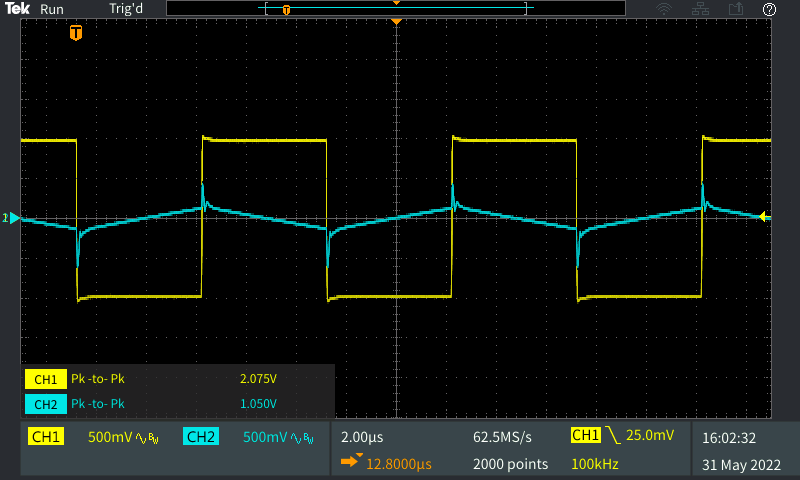
\includegraphics[width=1\linewidth]{./ImageFiles/Laboratorio 4/TEK00016}
	\caption{Confronto tra il segnale in ingresso v\sub{i} (CH1)  e in uscita v\sub{o} (CH2) all'integratore. In ingresso è stata applicata un'onda quadra di ampiezza \SI{1}{\volt} e frequenza \SI{100}{\kilo\hertz}.}
	\label{fig:opamp_int_quadra}
\end{figure}

\noindent
Infatti, un'onda quadra di ampiezza 1 e periodo T può essere definita come una funzione a tratti:
\begin{equation}
	f(x)=
	\begin{cases}
		1,\;se\;0<=x<T/2 \\
		-1,\;se\;T/2<=x<T 
	\end{cases}
\end{equation}
La sua funzione integrale $F(x)=\int_0^xf(t)dt$ è la seguente:
\begin{equation}
	F(x)=
	\begin{cases}
		x,\;se\;0<=x<T/2 \\
		T-x,\;se\;T/2<=x<T 
	\end{cases}
\end{equation}
che rappresenta proprio un onda triangolare.

\todo{vi nelgi opamp grande}